\section{WFB-FL 体系架构与端到端运作机制}
\label{sec:3}

为满足受控实验的收发要求，平台首先必须打通可控的无线收发能力，支持显式调节关键无线参数，并突破常规 Wi-Fi 对广播速率的限制。常规 Wi-Fi 很难做到这一点。商用固件全权接管物理层，在后台自行升降速率，并将广播帧锁死在低速的基本速率集。平台利用消费级网卡的 monitor 模式接收与原始帧注入绕过这一限制。开启 monitor 模式后，网卡脱离常规接入点的关联流程。通信对端直接捕获空中实际到达的无线帧，并记录随帧附带的 Radiotap 元数据，包括时间戳、工作频率、调制编码方案（MCS）索引与信号强度。原始帧注入则赋予发送端自主构造物理帧的能力。发送端越过操作系统内核的速率协商逻辑，把按指定参数组装的 802.11 帧直接送入无线信道。高阶物理速率的广播分发由此成为可能。

在此收发基础上，平台支持对六项关键无线参数实施显式设定，并依据不同的系统层次采用对应的配置途径。工作信道与频段、信道带宽以及发射功率，由网卡驱动与操作系统内核接口直接下发给射频芯片。决定单帧调制阶数与编码率的 MCS，以及用于抵御多径时延扩展的符号级保护间隔（GI），由发送端在构造原始帧时写入发射元数据，供物理层逐帧应用。用于抵御空口误码与突发丢帧的前向纠错（FEC），属于链路控制层对数据分组的冗余编码处理，由发送端为一组数据包附加密集校验块，与物理层编码配置处于不同层次。通信对端捕获到的物理帧与元数据，在下行由客户端记录，在上行由服务端记录，为后续实验提供直接的物理层核验依据。常规 802.11 广播机制本身缺乏逐接收端的硬件确认，而平台在虚拟网络接口之上依然复用成熟的网络协议。平台的核心任务是利用这些底层收发能力，为上层联邦学习构建可靠的一对多模型分发与有序的更新回传机制。

系统自上而下划分为五层（见 Fig.~\ref{fig:1}），各层职责边界分明。联邦学习算法层负责全局模型的训练评估与聚合逻辑。联邦学习运行层维护严格同步的训练轮次，编排模型发布、模型等待、更新提交与更新收齐。传输适配层承接模型与更新的文件交换需求，向下将其映射到具体传输协议，其中下行采用一对多文件分发协议 UFTP，上行采用 HTTP PUT 配合底层 TCP 传输。链路控制层以 TUN 虚拟网卡作为网络边界，管理发送许可、调度控制消息、出站发送队列与入站重组缓冲。无线收发层驱动无线网卡执行原始帧注入与 monitor 模式接收。调用自顶向下发起，完成结果逐层向上返回。TUN 虚拟网络接口承接上层普通数据流量，链路控制帧则由独立的控制通道直接传输，不经过 TUN 接口。

% 原稿标记保留：**[Figure 1 占位 WFB-FL 五层架构与简化端到端流程图]**

% 原稿题注保留：> Figure 1 展示服务端与多个客户端的五层职责划分、TUN 边界，以及模型下行、本地训练、更新上行与聚合的简化流程，并标明传输适配层在下行采用一对多文件分发协议 UFTP、在上行采用 HTTP PUT 与 TCP。

\begin{figure*}[tb]
\centering
% 裁去图稿上下的纯白外边距，保留所有图内元素；PDF 文件本身不变。
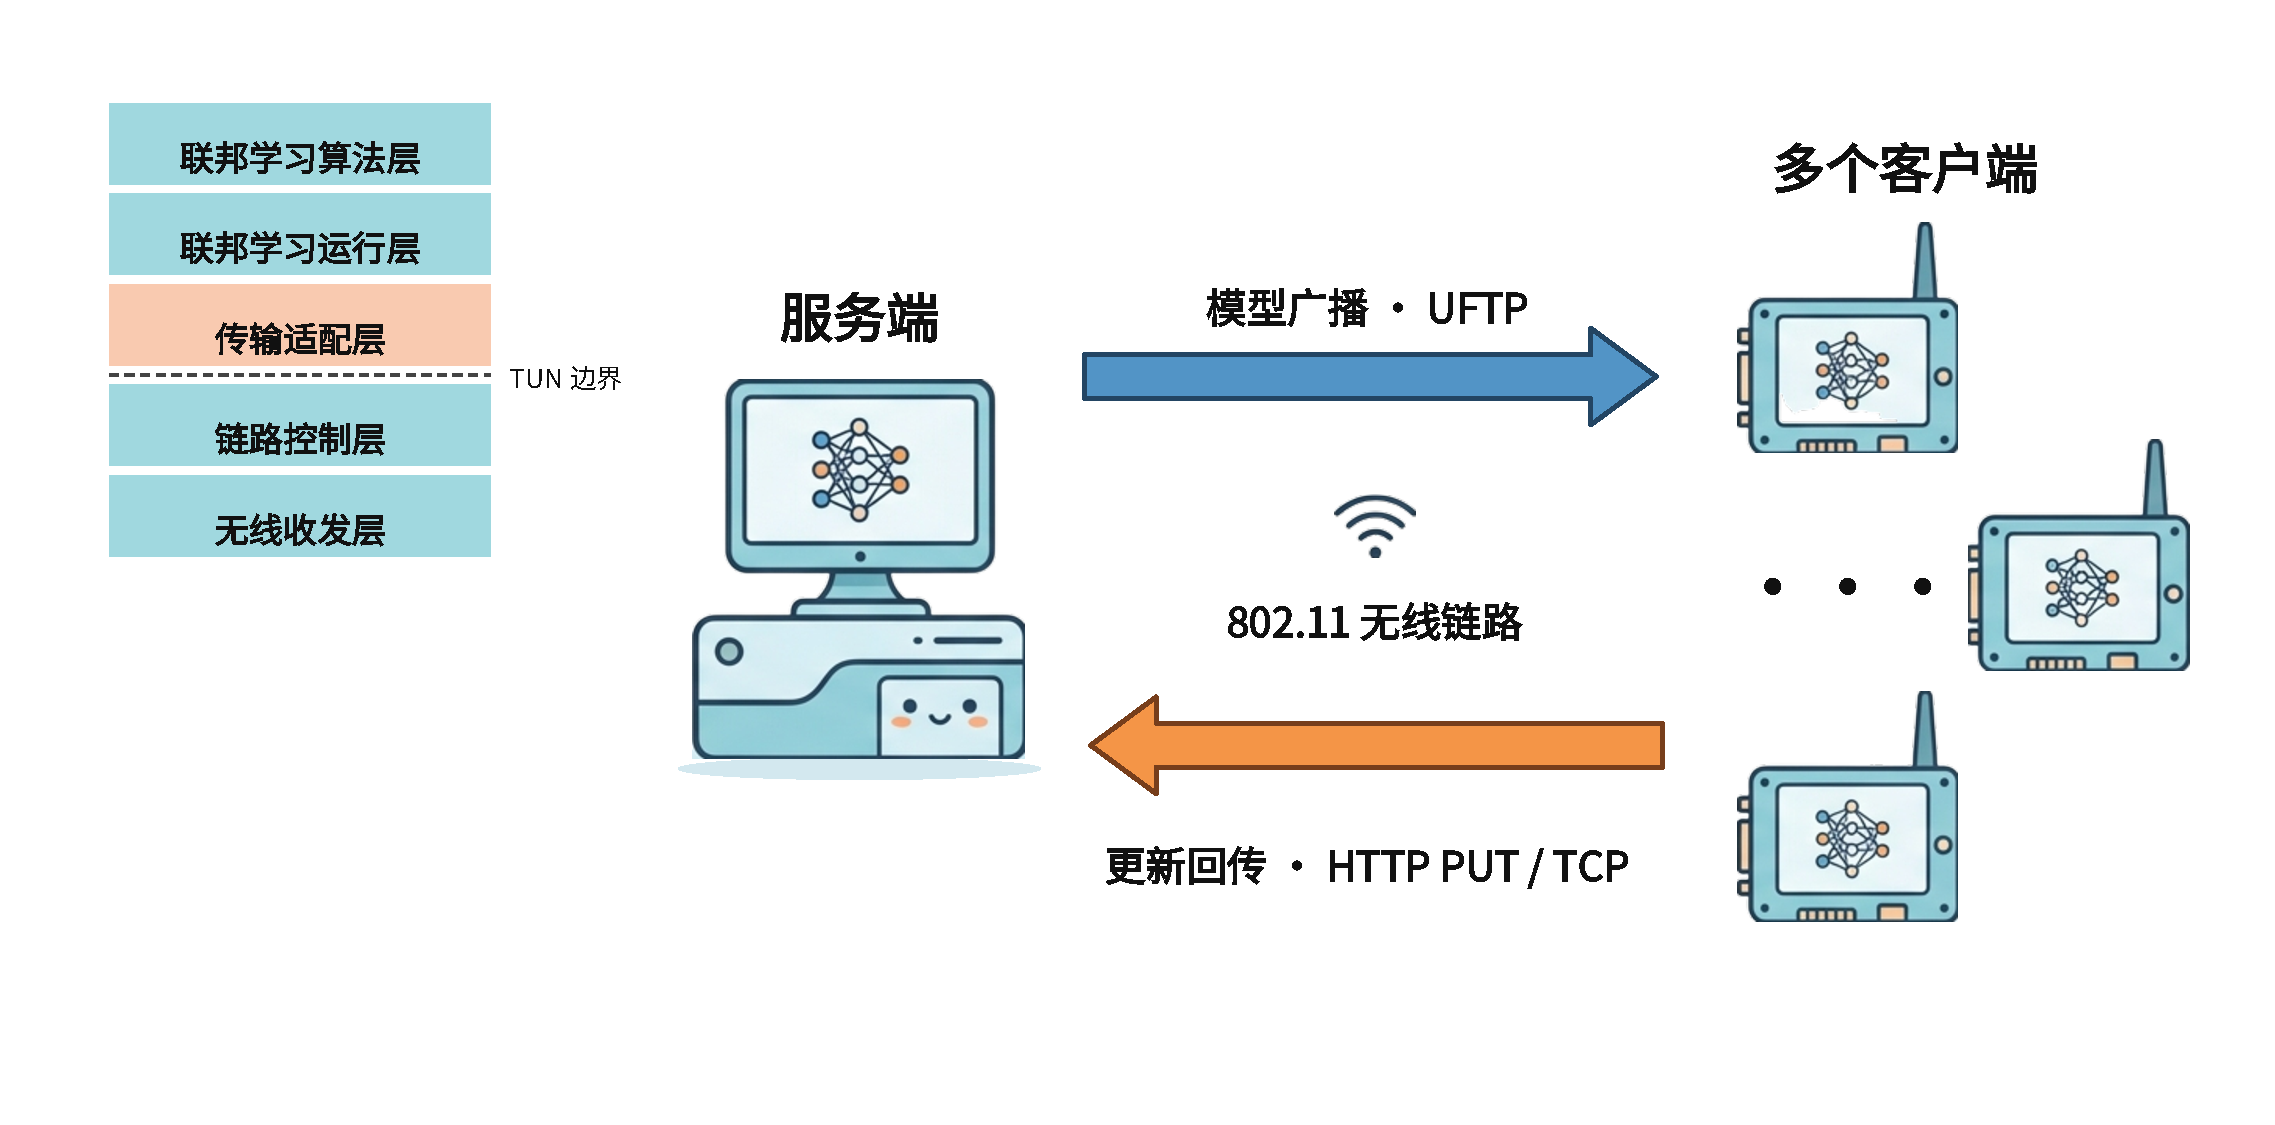
\includegraphics[width=\textwidth,trim=0 80bp 0 32bp,clip]{figure1.pdf}
\caption{WFB-FL 五层架构与简化端到端流程。}
\label{fig:1}
\end{figure*}

一轮联邦学习训练由服务端发起。算法层准备好全局模型，运行层冻结本轮参与训练的客户端集合并生成交付清单，交由传输适配层启动模型分发。下行传输选择一对多文件分发协议 UFTP。同一份全局模型要送到全体客户端手中，面对典型的一对多单向流量，直接复用成熟协议在分块、缺块反馈与选择性补发上的现成能力，可以省去重复实现复杂的可靠传输逻辑。高阶物理速率的无线广播由底层的原始帧注入直接提供，UFTP 则专注于在此广播承载之上保障文件交付的可靠性。广播帧在无线信道传输时可能因衰落或偶发干扰发生丢包，系统通过两道防线逐级恢复。第一道防线由链路控制层的前向纠错承担。发送端在分组层面附加纠错冗余块，客户端在接收到部分丢帧的情况下，只要成功捕获的分组数量达到恢复门限，即可在本地直接重构原始数据块。超出前向纠错恢复能力的个别缺块由第二道防线处理。客户端记录缺失数据块的编号并在反向反馈机会中告知服务端，服务端接收反馈后重新广播补发对应的数据块。

客户端回传缺块信息与完成状态时，多个客户端共享同一无线信道。多节点同时回传，信号必然在空中相互重叠与干扰。解决办法是发送权轮转（见 Fig.~\ref{fig:2}）。服务端定期暂停主广播，拿出当前活跃队列的快照，按顺序轮流给客户端发许可。许可对应一个固定时长的限时发送窗口。拿到窗口的客户端才能发数据，时间一到立刻停手。前后两个窗口之间还要留出固定的窗口切换间隔，留出足够的物理时间间隙，防止前后两台设备的无线信号发生交叠。发送权轮转机制旨在协调平台内部受管客户端的发送时机，有效降低彼此之间发生发送冲突与信号碰撞的可能。该机制并不改变开放无线环境的物理特性，无法阻止未受管外部设备的射频干扰，也不声称信道在物理层面上始终由单一节点独占。

% 原稿标记保留：**[Figure 2 占位 发送权轮转机制图]**

% 原稿题注保留：> Figure 2 解释限时发送机会在节点间的轮换过程、窗口到期停发特征以及相邻发送机会之间的窗口切换间隔。

\begin{figure*}[b]
\centering
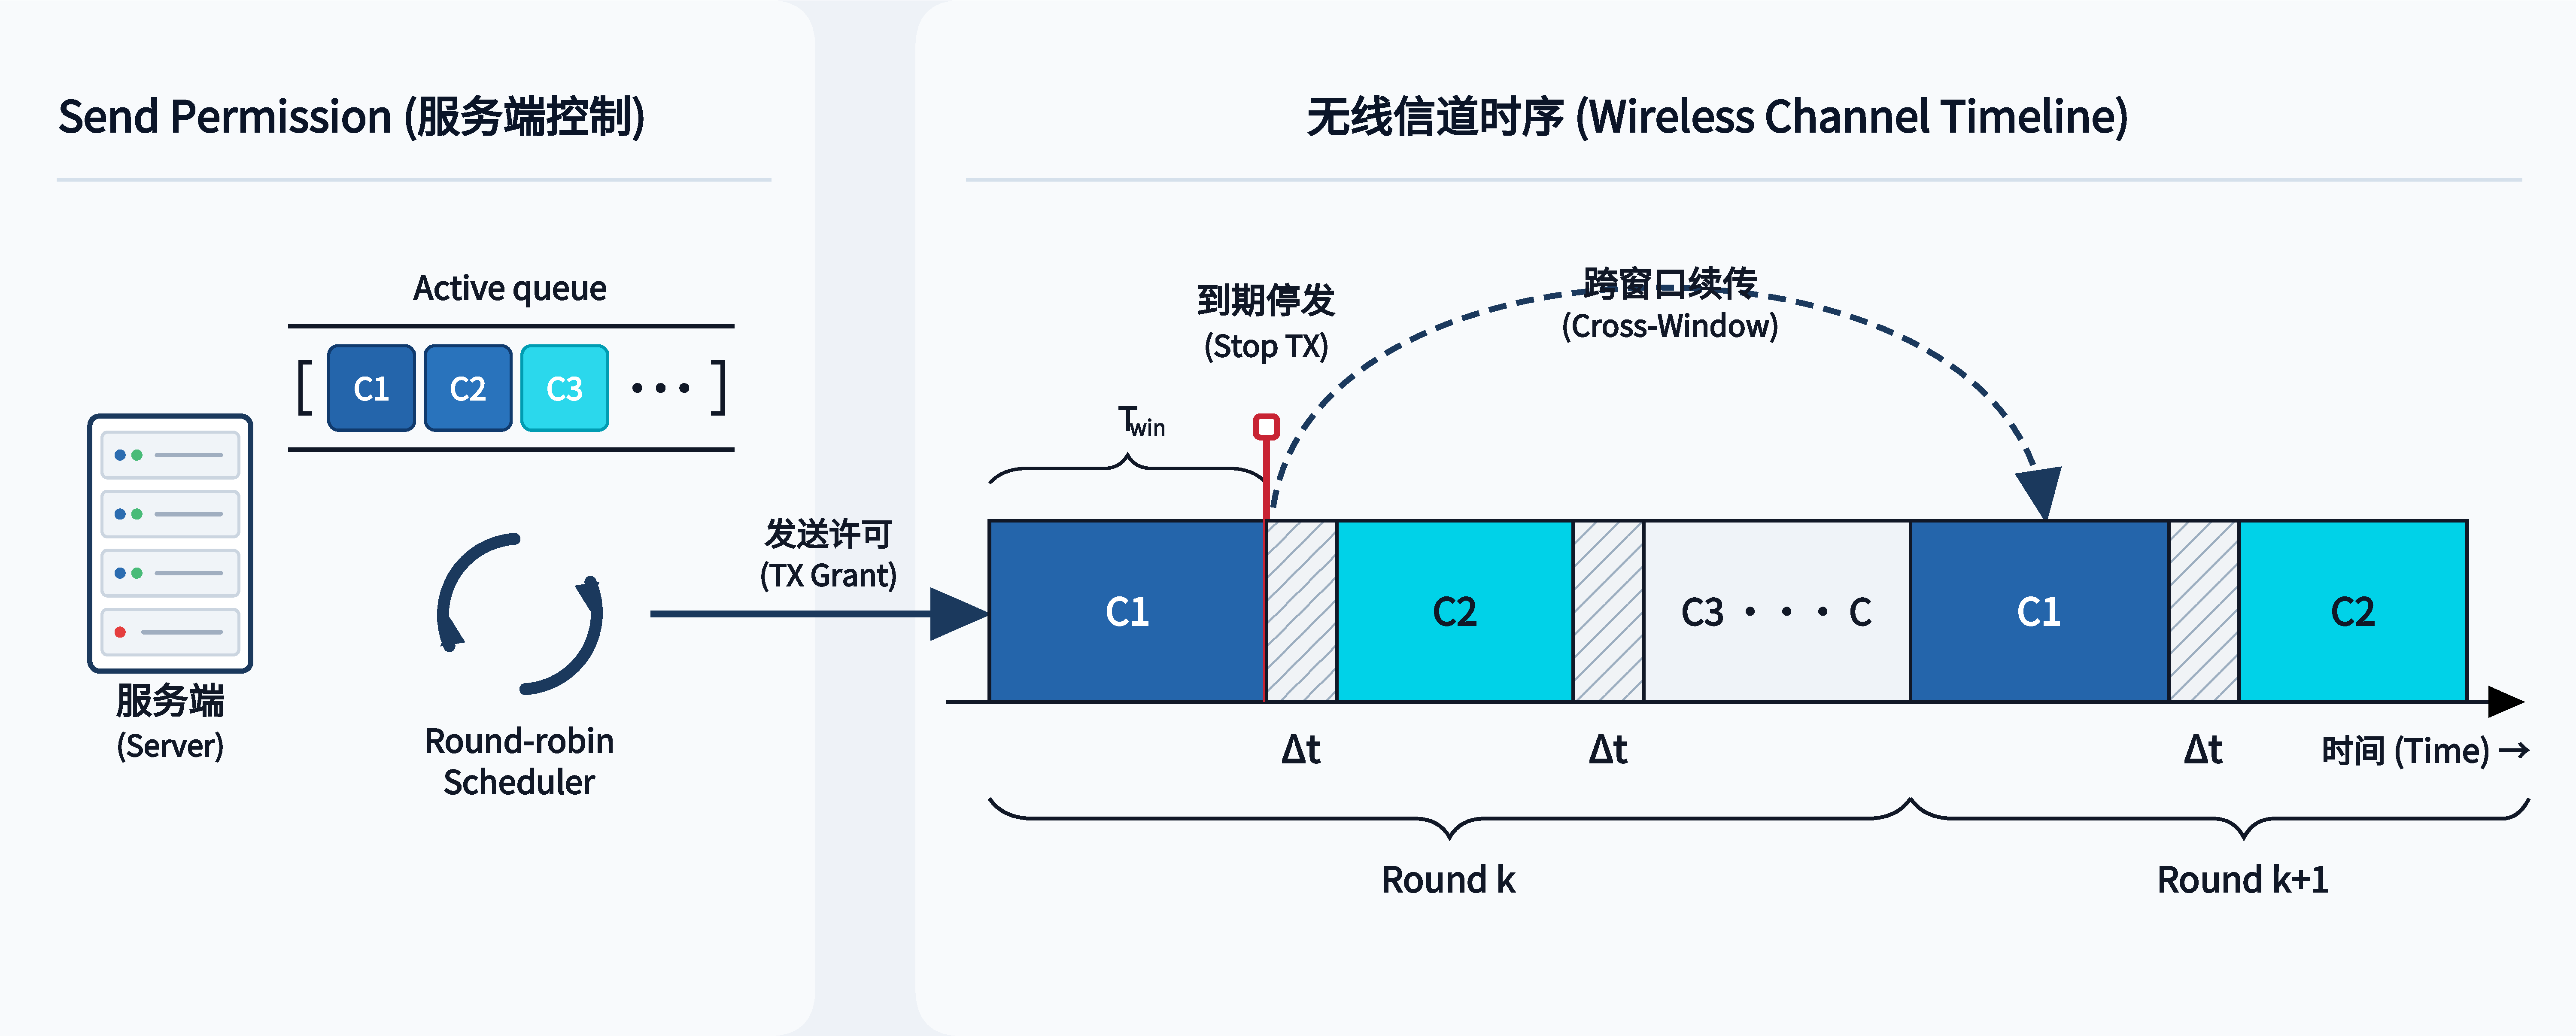
\includegraphics[width=\textwidth]{figure2.pdf}
\caption{发送权轮转与限时发送窗口。}
\label{fig:2}
\end{figure*}

下行阶段的结束包含客户端与服务端两个层次的完成判定。任何一个客户端在本地通过 UFTP 接收到完整模型文件，并通过运行层的格式与 SHA-256 摘要校验后，即可立即返回模型路径并启动本地训练，不必等待其他客户端同步完成。服务端的运行层则必须等待传输适配层确认全部预期目标客户端均已可靠收到模型文件，方才越过下行完成屏障。下行完成屏障只约束服务端的模型发布判定，为全局轮次立下交付基线；只要本地校验通过，客户端尽可直接进入训练，不必受其约束。

客户端完成本地模型训练后，生成各自的更新文件并进入更新回传阶段。各客户端本地训练产生的数据更新各不相同，属于典型的多对一独立文件提交，上行传输因而选择 HTTP PUT 配合底层 TCP 协议。HTTP PUT 提供了成熟的请求响应语义、内容长度界定与状态码规范；底层的 TCP 协议则保证了字节流可靠有序。平台在传输适配层中额外执行客户端身份核验、文件长度比对与数据摘要验证，确保更新文件的完整性，不把全部校验责任推给 HTTP 协议本身。客户端更新数据进入链路控制层的发送队列后，队列由空变为非空触发客户端向上发送就绪声明。服务端完成合法性校验后将客户端加入活跃队列，并复用下行建立的发送权轮转机制（如 Fig.~\ref{fig:2} 所示），按顺序轮流为客户端授予限时发送窗口。上行传输同样依靠链路层前向纠错抵御无线丢包，剩余的字节流缺失则由 TCP 的确认与重传机制处理。在各客户端的普通上行发送机会之间，服务端保留短暂的反向传输机会以回传 TCP 确认帧，保证双向流控正常推进，该反向机会不同于下行 UFTP 的周期性反馈轮。

客户端模型更新文件体积通常达到数十兆字节，远超单个发送窗口所能承载的容量，必须跨越多个限时发送窗口持续推进。单次窗口到期只是暂停网卡的无线发送。传输适配层已经建立的 HTTP 连接依然维持，未发完的请求也不会撤回；待发数据留在本地发送队列中，等下一个许可窗口打开，接着往前传，不用重建连接，更不用重发数据。仅当发生网络超时或物理连接断开时，系统才按传输契约判定失败，并不承诺任何异常下连接绝对不中断。

链路控制层维护固定容量的用户态出站发送队列，承接已从 TUN 读取但尚未发出的数据面流量。为防止数据源源不断注入导致队列无限膨胀乃至内存耗尽，系统设置高低两道字节积压水位以及数据包数量硬上限。当队列中积压的待发字节达到高水位阈值时，链路控制层主动暂停从 TUN 虚拟网卡读取新数据，通过系统网络栈自身的流控机制向上层应用形成反压。当积压数据随空口发送减少、降至低水位阈值后，系统重新恢复从 TUN 读入。双阈值构成的滞回区间可有效避免临界点上的频繁启闭（见 Fig.~\ref{fig:3}）。数据包数量硬上限独立发挥作用，防止大量小尺寸数据包在未触碰字节水位前耗尽队列索引。相同的队列容量约束、双水位滞回与反压机制，同样适用于服务端的下行数据发送。此处起伏变化的是随传输节奏波动的队列积压量，阈值本身属于静态预设参数，并不存在随链路状态自动调整的复杂算法。

% 原稿标记保留：**[Figure 3 占位 队列水位与反压机制图]**

% 原稿题注保留：> Figure 3 解释出站发送队列的字节积压变化，以及达到高水位暂停从 TUN 读入、降至低水位恢复读入的反馈调节关系。

\begin{figure*}[t]
\centering
% 裁去图稿上下的纯白外边距，保留所有图内元素；PDF 文件本身不变。
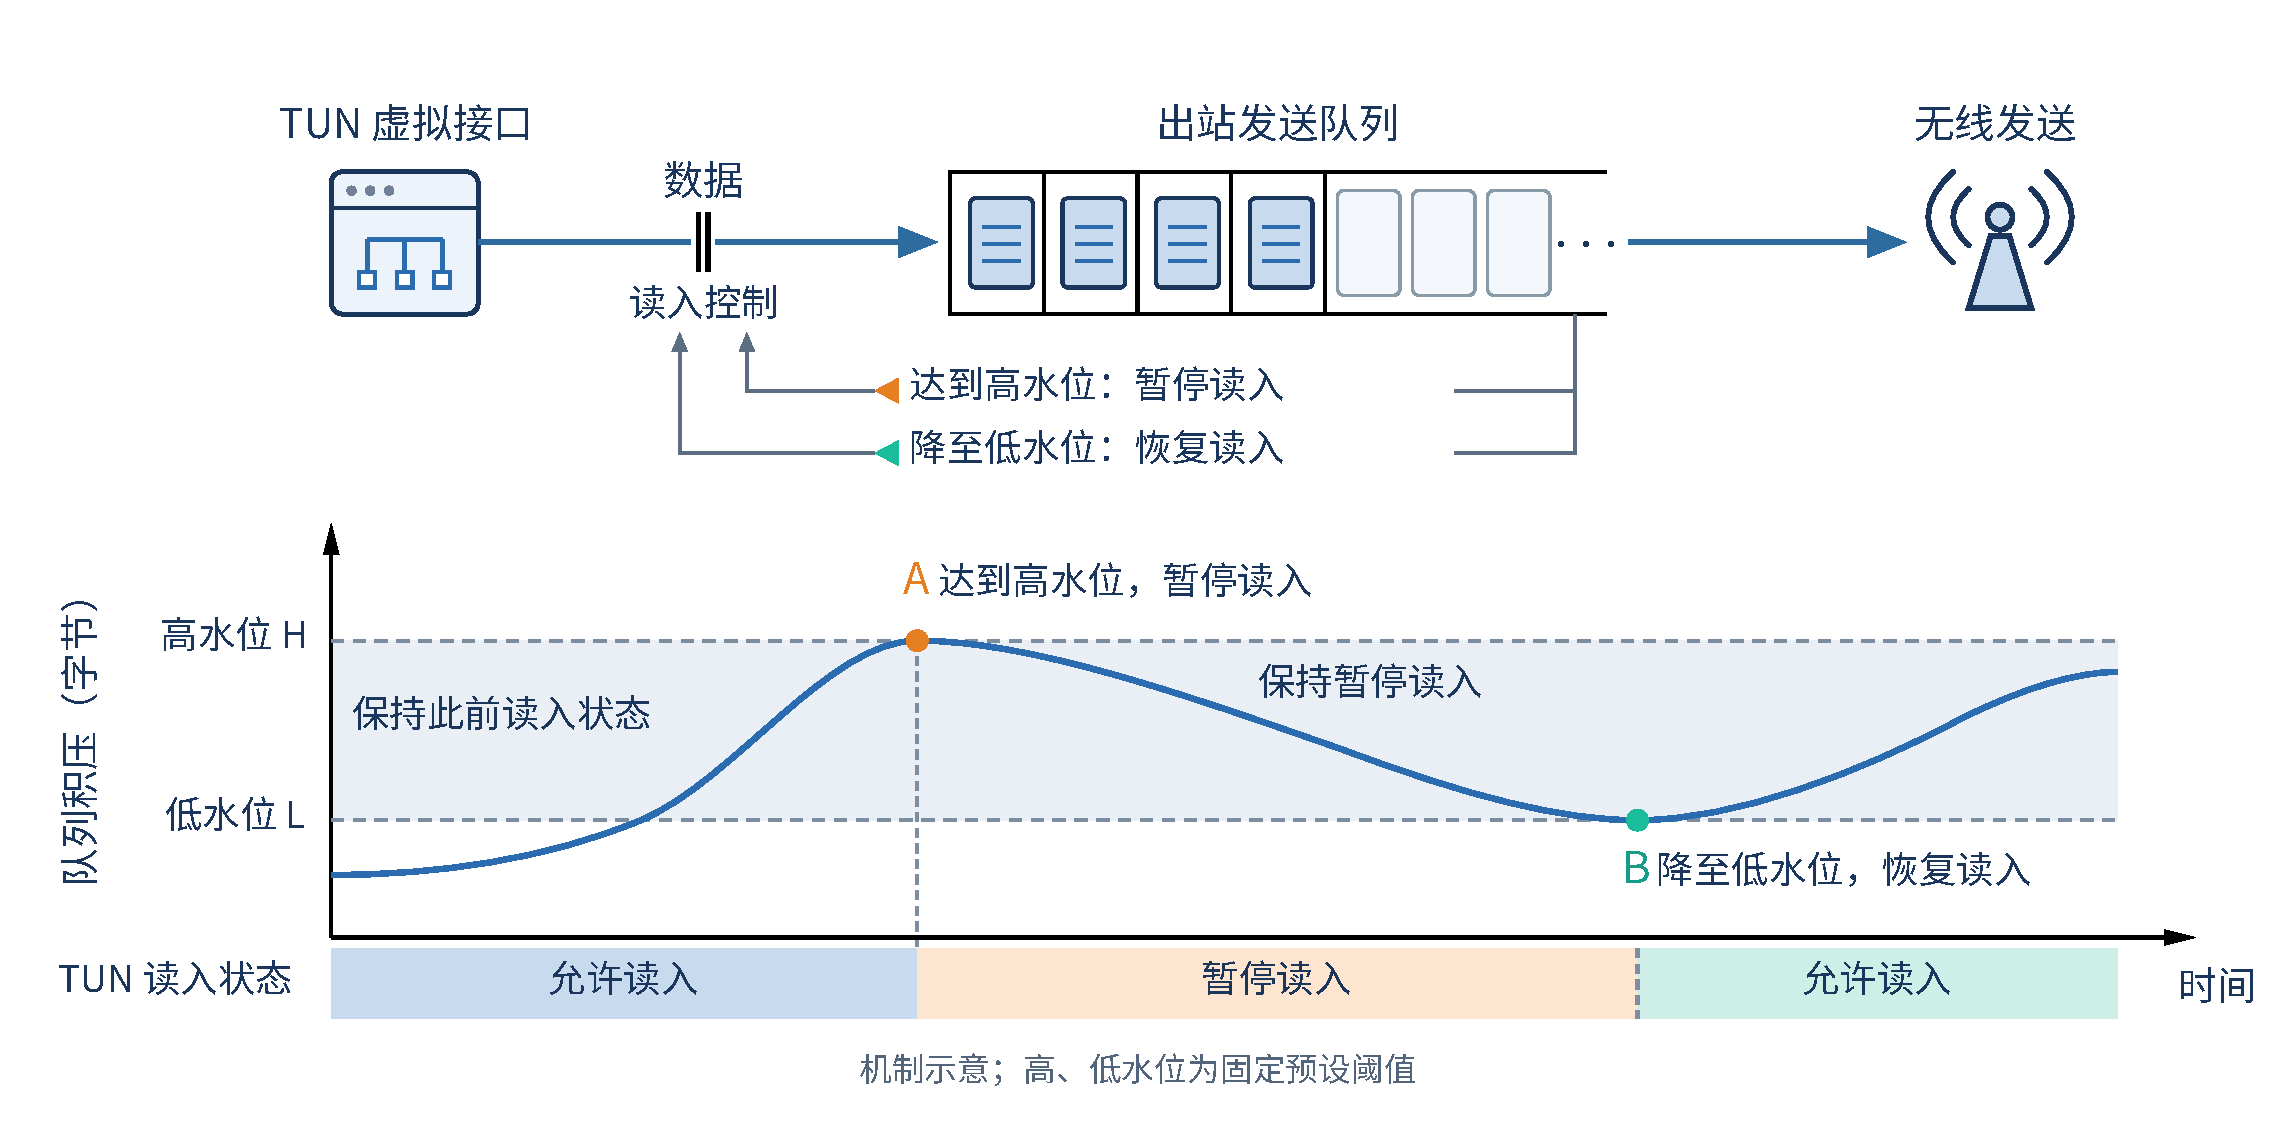
\includegraphics[width=\textwidth,trim=0 2bp 0 32bp,clip]{figure3.pdf}
\caption{出站发送队列的双水位反压机制。}
\label{fig:3}
\end{figure*}

就绪声明与发送许可等链路调度控制消息走独立的优先通道，直接经由无线收发层收发，不进入出站发送队列，也不经过 TUN 接口。即使普通数据队列处于高水位积压或处于反压停读状态，调度控制帧依然可以顺畅收发，避免大文件传输阻断调度控制。出站发送队列与入站接收重组缓冲在职责上保持独立。出站队列承接本机向外发送的数据，入站接收重组缓冲则承接从无线信道接收的数据分片，负责处理乱序到达、分组缺片以及前向纠错恢复。多个客户端交替上行时，服务端接收端根据每个无线分片中携带的发送者身份标识，对不同客户端的数据块分别进行隔离重组，防止多节点数据混合错乱。接收重组缓冲的积压或淘汰同样独立于控制通道，不能影响调度控制消息的正常收发。

一轮训练的最终收束涉及多层完成判定的协同，各层边界不可相互替代。发送许可生效仅代表客户端取得了在无线信道上的发送机会。服务端 monitor 模式捕获到无线帧仅证明物理信号到达本机，不等于上层接收到合法文件。单个客户端的更新文件在传输适配层通过长度比对与 SHA-256 摘要核验，并在服务端存储路径完成原子文件提交后，才构成该客户端更新文件的正式提交。服务端运行层在确认下行完成屏障已经达成、且本轮预期的全部有效客户端更新文件均已完整收齐后，才将全部更新文件打包交付联邦学习算法层执行全局模型聚合。单个客户端提交成功绝不等于整轮联邦学习成功，只有全部有效更新完整入库才能驱动算法层完成本轮训练。
